\documentclass[journal]{IEEEtran}
\usepackage{amsmath,amssymb,booktabs,cite,graphicx}
\usepackage[hidelinks]{hyperref}
\begin{document}
\raggedbottom
\title{Matched-Budget Boundary Refinement for SAR Ship Instance Segmentation}
\author{Author~Details~Pending\thanks{Internal review draft. Author affiliations and submission metadata are pending.}}
\maketitle

\begin{abstract}
A one-pixel shift can leave the area of a narrow synthetic aperture radar (SAR) ship mask intact and remove much of its overlap with the annotated vessel. We fit a 1,321-parameter point head to source polygons and compare two ways of choosing additions and removals on the original image grid. At the same endpoints, scores, and counts on each side, independent selection raises mask average precision (AP) over distance pairing by 0.81--0.91 points across one D-FINE and two RF-DETR fits on 705 HRSID development images. The gain is 1.22 points on the historical HRSID official split and 0.48 and 0.30 points in two frozen RF-DETR transfers to 583 Gaofen-3 images. With pretrained Phoenix probabilities, capping whole-image updates recovers 9.39 AP on 74 Instance-RSDD chips and 2.52 AP on 232 PSeg-SSDD images relative to thresholding. On PSeg-SSDD, equalizing additions and removals on the sampled endpoints raises AP by 1.84 points relative to the free allocation on those same endpoints. Balanced Phoenix reaches 18.22 AP, compared with 18.42 for matched static spatial attraction.
\end{abstract}
\begin{IEEEkeywords}
Synthetic aperture radar, ship instance segmentation, boundary refinement, native image grid.
\end{IEEEkeywords}

\begin{figure*}[!t]
\centering
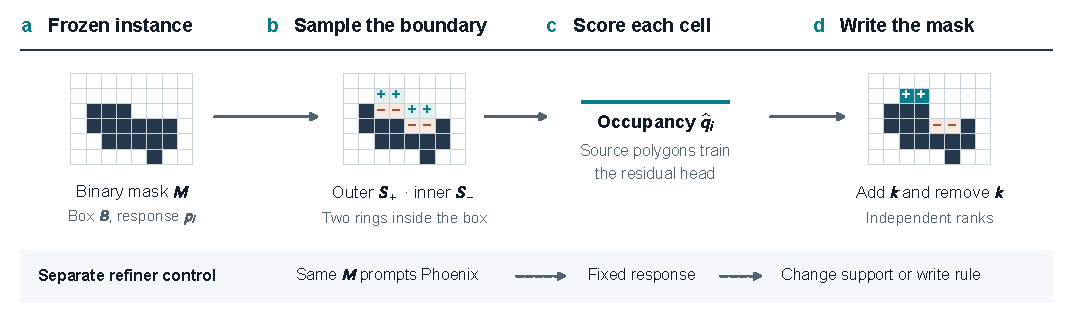
\includegraphics[width=\textwidth]{figures/matched_budget_pipeline.pdf}
\caption{Native-grid boundary refinement. (a) A frozen prediction supplies the mask, box, score and decoder response. (b) Source polygons supervise a residual point head through fractional cell occupancy. (c) The two writers share the same signed endpoint sets and occupancy scores. At count \(k\), fixed pairing selects entire distance-assigned pairs, and independent selection ranks additions and removals separately. Each writer adds and removes \(k\) cells. The grid, scores and edits are schematic.}
\label{fig:native-boundary}
\end{figure*}

\section{Introduction}
A one-cell transverse shift of an ideal four-cell-wide ship gives an intersection over union (IoU) of 0.60, even though the two masks have identical area. More generally, a rectangle \(w\) cells wide gives \((w-1)/(w+1)\) after the shift. Uneven scattering, speckle, and nearby structures can obscure the boundary of an actual SAR ship. Stronger object features and rotated regions improve the upstream proposals \cite{gao2024,aranet,drsnet}. Here we examine the remaining boundary error when the proposal and its confidence are already given.

An oracle on 1,329 fixed matches of small, slender ships in the HRSID~\cite{hrsid} development set illustrates the distinction between support and placement. A two-pixel box expansion makes continuous IoU 0.90 attainable in 134 additional cases. Keeping the original foreground and permitting additions only outside the original box reaches 0.90 in zero of those cases. Repositioning existing foreground is therefore necessary in this diagnostic. The reference is the annotated SAR footprint. Its agreement with the physical hull is a separate measurement question.

Suppose a boundary writer may add \(k\) pixels and remove \(k\). A distance-based assignment links each addition to one removal. Independent selection can keep the best-scored additions and removals even when they belong to different assigned pairs. We compare these two choices using a common set of endpoint scores learned from fractional overlap with the source polygons. Removing the pairing restriction increases the maximum \emph{estimated} intersection gain. The measured result depends on the ordering errors of the predictor. A clutter cell can score above a true boundary cell, in which case the additional freedom can reduce overlap.

We make three comparisons at the original image resolution.
\begin{enumerate}
\item We fix the predicted mask, endpoint locations, scores and per-candidate edit count to measure the effect of distance-based pairing on two detector families.
\item We train a source-only fractional occupancy predictor and compare its rankings with geometric attraction and published refiners. Equal-support comparisons and complete-mask outputs expose distinct effects of the score and the writer.
\item We cross writable support and edit count on two public benchmarks using frozen Phoenix probabilities. The paired geometry, actual pixel changes, and missed matches explain when limiting edits recovers overlap and where performance still trails the native detector.
\end{enumerate}

\section{Related Work}
PointRend~\cite{pointrend} adds detail during mask subdivision by querying decoder features at selected points. Boundary Patch Refinement~\cite{bpr} revisits patches around an existing outline, and RefineMask~\cite{refinemask} carries coarser stage predictions forward outside the refined boundary band. SharpContour~\cite{sharpcontour} moves contour vertices with instance-conditioned point predictions. SegFix~\cite{segfix} assigns boundary labels from corresponding interior pixels. Phoenix~\cite{phoenix} learns to reconstruct progressively perturbed prompt masks. We evaluate the published refiners on their own writable regions and compare their rankings with the same editable locations and quota. For PointRend we also preserve the sign counts and exterior edits of its whole-region paste while replacing locations within the sampled support.

Atkinson~\cite{atkinson} ranks foreground and background subpixels separately to preserve class proportion within each coarse land-cover cell. Xu and Huang~\cite{xu} score subpixel pairs using spatial and temporal data. RankSEG~\cite{rankseg} derives posterior ranking and foreground-volume selection for IoU and Dice. These results motivate the use of separate ranks. In an existing ship mask the paired writer already implies a realized count for that particular candidate. Holding that count and the estimated occupancies fixed yields a direct test of the distance assignment on the native grid.

In SAR segmentation, Gao et al.~\cite{gao2024} use dynamic key points from strong scattering regions, and DRSNet~\cite{drsnet} improves local features in rotated regions. GLDet~\cite{gldet} combines global context with local gradients upstream of the detection and mask outputs. DACF-Net~\cite{dacf}, GCIE-Net~\cite{gcie}, DSR-Net~\cite{dsr}, and ARANet~\cite{aranet} also change learned representations and may change which vessels appear in the candidate list. We freeze the proposals of D-FINE-seg~\cite{dfine} and RF-DETR~\cite{rfdetr}. The polygon coordinates of HRSID and the pixel instance segmentation release of SSDD (PSeg-SSDD)~\cite{ssdd} allow direct overlap measurements on the resulting small footprints.

\section{Method}

\subsection{Boundary samples on the native image grid}
We refine one detected instance at a time. The detector supplies a binary mask \(M\), a box \(B=[x_1,x_2)\times[y_1,y_2)\), a confidence \(s\), and a decoder response. All coordinates refer to the decoded image. The cell indexed by \(i=(x,y)\) occupies \(C_i=[x,x+1)\times[y,y+1)\). The mask defines the foreground. A candidate edit at \(i\) is an addition if \(M_i=0\) and a removal if \(M_i=1\). Instance identities, boxes, class labels, and confidence scores are fixed throughout refinement.

The two detectors supply different point features. For D-FINE, we sample the \(160\times160\) pre-crop sigmoid probability plane at native cell centers. The sampler rounds the plane to half precision, performs bilinear interpolation in single precision with half-pixel coordinates, and rounds the sampled value to half precision. For RF-DETR, bilinear interpolation with half-pixel coordinates acts on the raw mask logits before the sigmoid. We denote the resulting foreground response by \(p_i\). The stored native mask determines the edit sign throughout, including any disagreement between its binary decision and the sampled response.

For masks with \(32\leq |M|<1024\), two successive dilations and erosions with a \(3\times3\) square define the outer and inner boundary bands. Morphology uses a zero exterior. Integer column and row indices must belong to the native image and to \(B\). If the bands contain \(n_+\) background and \(n_-\) foreground cells, we keep \(n=\min(32,n_+,n_-)\) per side. Selection is by increasing \(|p_i-0.5|\), with ties resolved by native row-major index. This yields the addition set \(S_+\) and removal set \(S_-\). Masks outside the area range, or with an empty side, pass through unchanged. For the paired comparison, a minimum-cost bipartite assignment joins the two sets using squared Euclidean distance between cells (Fig.~\ref{fig:native-boundary}).

\subsection{Learning fractional cell occupancy}
For a source detection matched to a valid reference polygon \(G\) at raster IoU 0.50, the supervision for cell \(i\) is \(q_i=|C_i\cap G|/|C_i|\). A contour that crosses a cell therefore contributes its measured area fraction. The 14 features are \(p_i\), the original foreground indicator, boundary-layer index, Euclidean distance to the opposite mask class, two box-relative coordinates, \(\log_2|M|\), box fill fraction, \(s\), grayscale intensity, its \(3\times3\) and \(5\times5\) means, and two centered intensity differences. Intensities come from the decoded RGB rendering.

Let \(z_i\) be the standardized feature vector. We compute first and second moments within each training source group, then average those moments across groups. Write \(\widetilde p_i\) for \(p_i\) clipped to \([10^{-4},1-10^{-4}]\). The point head estimates
\begin{equation}
 \widehat q_i=\sigma\!\left[\operatorname{logit}(\widetilde p_i)
       +f_\theta([z_i,z_i])\right].
\end{equation}
The two hidden layers of \(f_\theta\) each have 24 ReLU units. Initializing the scalar output layer with zero weights and bias makes the initial prediction equal to the clipped decoder response. Duplicating \(z_i\) gives the 1,321-parameter head the same input dimension as the partner-feature controls. Both occurrences describe the same cell in the principal model. Training minimizes binary cross-entropy with fractional targets on both cells of each sampled pair. Each of the 200 AdamW updates uses 64 pairs, learning rate 0.002, and weight decay 0.01. A draw samples a source group uniformly, then a pair uniformly within that group. In the five-fold FIT109 development experiment, normalization and head fitting exclude the held-out source prefixes. For HRSID-to-target transfer, we refit on the complete source training bank and retain those normalization constants and weights.

\subsection{Paired and independent location selection}
Write \(P=|M|\), \(T=|G|\), \(I=|M\cap G|\), and \(U=P+T-I\), interpreting \(M\) as the union of its foreground cells. Adding \(A\subseteq S_+\) and removing \(D\subseteq S_-\) changes intersection by \(g=\sum_{i\in A}q_i-\sum_{i\in D}q_i\) and foreground area by \(d=|A|-|D|\), in native pixel-area units. Equal counts give \(d=0\) and
\begin{equation}
 \frac{I+g}{U-g}-\frac{I}{U}=\frac{(P+T)g}{U(U-g)} .
 \label{eq:gain}
\end{equation}
Thus the intersection gain determines the ordering of feasible equal-area edits for that instance. With unequal counts, the union becomes \(U+d-g\), giving
\begin{equation}
 \Delta\mathrm{IoU}=\frac{(P+T)g-Id}{U(U+d-g)} .
 \label{eq:variable-area}
\end{equation}
Normalized false-positive and false-negative areas are \((P-I)/T\) and \((T-I)/T\). After editing they become \((P+d-I-g)/T\) and \((T-I-g)/T\), respectively.

The paired policy scores each assigned pair \((a_j,d_j)\) by \(\widehat q_{a_j}-\widehat q_{d_j}\). It takes pairs in descending order while the gain is positive, up to \(K=\min(8,\lfloor P/10\rfloor,n)\). Its realized count \(k\) can be zero. The matched independent policy inherits this \(k\) for the same instance. It chooses the \(k\) largest addition scores and \(k\) smallest removal scores, resolving ties by the original endpoint ordinal. This maximizes the estimated intersection gain over all such choices, including every choice available under the assignment. In particular, an addition selected from one assigned pair can accompany a removal from another. Equation~\eqref{eq:gain} applies to the true polygon fractions, so a gain in the predicted objective can still cost reference overlap. Its effect on mask AP also depends on confidence ordering and threshold-specific matching across the candidate pool. In the natural-count comparison, independent selection stops when the next independently ranked pair has nonpositive gain or the same cap \(K\) is reached.

\subsection{Support and flip rules for the pretrained refiner}
We separately evaluate Phoenix XL1~\cite{phoenix} with the original binary mask as prompt. After five refinement iterations, we use the selected mask hypothesis and its native-resolution foreground probability \(r_i\). The reference count \(k_{\rm att}\) is inherited from dynamic spatial attraction~\cite{atkinson}. It computes foreground attraction with weights \(\exp(-\rho/5)\) at distances \(0<\rho\leq5\) native pixels and updates the attraction after each positive-gain exchange, subject to the same cap \(K\). The writable support is either \(S_+\cup S_-\) or the whole native image. On either support, the threshold rule writes all disagreements between the author's binary output and \(M\). The count rule makes exactly \(2k_{\rm att}\) flips. It ranks additions by \(r_i-0.5\) and removals by \(0.5-r_i\). For each feasible split between the two sides, the objective sums the leading margins on both sides. Equal-utility splits favor the smallest absolute net area change, then fewer additions. To isolate the split itself, a further comparison assigns \(k_{\rm att}\) flips to each side on the sampled endpoints and keeps the same within-side ranks. Fixed quotas can include nonpositive margins. Within a sign, ties follow the original endpoint order, followed by row-major order outside the sampled support. We calculate the interaction by subtracting the narrow count-minus-threshold contrast from the whole-image contrast. Every Phoenix comparison preserves the detections and scores. Instances with zero realized budget retain their original masks.

\section{Experimental Protocol}
\subsection{Data and Metrics}
The HRSID-trained detector and point head are frozen before transfer to Instance-RSDD, PSeg-SSDD and UEIKAP (Table~\ref{tab:cohorts}). In a separate PSeg experiment, we fit a target head while retaining the same PSeg-trained detector used with the source head. UEIKAP releases outlines for selected hulls. We measure coverage and outline overlap for those hulls.

\begin{table*}[t]
\centering
\caption{Evaluation cohorts and reference scope. The Gaofen-3 and date-separated views are nested within their respective Instance-RSDD cohorts. Source-prefix groups on HRSID are proxies for acquisition.}
\label{tab:cohorts}
\footnotesize
\setlength{\tabcolsep}{5pt}
\begin{tabular}{@{}lrrp{0.43\textwidth}@{}}
\toprule
Cohort & Images & Outlines & Evaluation role \\
\midrule
HRSID DEV705 & 705 & 1,782 & Detector-held-out source development, 27 source-prefix groups with prior development exposure. \\
HRSID official & 1,962 & 5,922 & Historical official allocation, with overlap and empty-raster checks. \\
Instance-RSDD author test & 740 & 872 & Frozen HRSID transfer, 112 author acquisition groups. Gaofen-3 view: 583 images, 631 outlines, 76 groups. \\
Instance-RSDD author train reserve & 74 & 81 & Frozen HRSID transfer on 13 additional parents. The date-separated view uses 42 images from eight parents. \\
PSeg-SSDD historical official & 232 & 546 & Frozen HRSID transfer with original decimal polygons. A 222-image sensitivity excludes historical same-data overlap. \\
UEIKAP reserve & 108 & 139 & Targeted author hulls from 18 Sentinel-1 acquisitions. \\
UEIKAP additional acquisitions & 342 & 528 & Targeted author hulls from 13 Sentinel-1 acquisitions. \\
\bottomrule
\end{tabular}
\end{table*}

The D-FINE E24 detector was trained on 2,937 HRSID images from the official training split. The point head was developed with five-fold source-prefix cross-fitting on FIT109 within that population, then refitted and frozen before target evaluation. DEV705 comprises 705 images with zero exact encoded or RGB-content overlap and no filename-source-prefix overlap with FIT. The filenames are proxies for acquisition groups, and DEV705 has prior development exposure.

The HRSID official PNG test split contains 1,962 images and 5,922 annotations. Four annotations rasterize to empty masks. Two test images match FIT exactly and one pair within the test split is identical. Before scoring, we fixed a primary evaluation on the full set and sensitivities excluding the four empty raster annotations or the three exact-identity images. The project previously used this split for model selection. We report the frozen reevaluation as a historical comparison on the official allocation.

COCO mask AP, AP75, AP90, small-mask AP and AR100 use the full candidate stream. For geometric analysis we retain each original nonignored raster-IoU-0.50 association and intersect the edited mask's native cells with the matched reference polygon. A change in AP can therefore reflect a different association, whereas a change in fixed-match IoU concerns the original hull. For paired intervals we average eligible hulls in each represented group and resample the groups. With two or more point heads on the same detector and match set, we average their effects within each group first. AP seed ranges summarize the observed fits.

The HRSID RF-DETR fixed-match counts use continuous IoU \(>0.90\). The D-FINE source and DEV705 counts and PSeg RF-DETR counts include equality. COCO AP90 is computed independently from full-candidate raster matching. Our overlap sensitivity test retains COCO ordering, matching and area bins and replaces only the overlap matrix on common annotation support.

\section{Results}
\subsection{Effects of Pairing on HRSID}
\begin{table*}[t]
\centering
\caption{D-FINE E24 on HRSID DEV705. COCO AP and recall use all 70,500 original candidates. Continuous IoU gives equal weight to source groups over 1,447 eligible valid matches of 1,652 original fixed matches. All rows retain candidate ranks, scores and foreground areas. Scores are scaled by 100.}
\label{tab:dev}
\begin{tabular}{lrrrrrr}
\toprule
Mask policy & AP & AP75 & AP90 & Small AP & AR100 & Continuous IoU\\
\midrule
Raw D-FINE E24 & 48.160 & 51.507 & 0.145 & 47.196 & 54.018 & 75.798\\
Same head, fixed pairing & 48.916 & 53.453 & 0.146 & 48.017 & 54.792 & 76.258\\
Independent selection, fixed-pair count & 49.726 & 55.285 & 0.200 & 48.923 & 55.617 & 76.787\\
Independent selection, natural count & \textbf{50.715} & \textbf{57.760} & \textbf{0.223} & \textbf{50.034} & \textbf{56.695} & \textbf{77.217}\\
Native decoder ranking, natural count of independent policy & 47.951 & 50.616 & 0.126 & 46.927 & 53.765 & 75.652\\
\bottomrule
\end{tabular}
\end{table*}

The natural policy increases mask AP by 2.555 points and small-object AP by 2.838 points over raw D-FINE (Table~\ref{tab:dev}). Group-equal continuous IoU increases by 1.419 points, with paired 95\% interval \([1.265,1.587]\). All three original valid strict matches are retained, and 12 additional matches reach 0.90. COCO AP90 remains low in absolute terms.

At 83,059 swaps on 20,741 candidates, independent selection gains 0.811 AP and 0.529 continuous IoU over fixed pairing (IoU interval \([0.455,0.597]\)). The analogous five-fold FIT109 gains were 1.576 AP and 0.615 IoU. Natural selection makes 194,052 swaps, changing both coverage and count. Native decoder ranking at this count can force swaps with nonpositive predicted gains.

On 412 detector-visible FIT109 matches, truth-ranked geometry reaches IoU 0.90 for 11 with fixed pairing, 27 with independent equal counts, and 38 with free add and delete counts. These are bounds on the original support. Limited gains from partner features and direct difference supervision at matched counts motivated the simpler occupancy head.

Our Atkinson adaptation~\cite{atkinson} uses a five-pixel radius and decay length. At 43,624 dynamic swaps on 6,159 FIT109 candidates, learned, dynamic and static ranks scored 53.344, 48.152 and 48.669 AP. Learned gains over dynamic were 1.104 IoU (\([0.788,1.446]\)) and \(-0.164\) AP90. Keeping each neighbor's gray-rank affinity gained 1.519 AP and 0.165 normalized intersection (\([0.080,0.264]\)) over averaging equal-distance affinities. Gray rank alone and learned occupancy gained 0.370 and 3.039 AP over aligned affinity. FIT109 trained the detector. Heads used five source-held-out folds.

On detector-held-out DEV705, the frozen all-FIT109 head and both attraction rules exchanged 262,802 pairs on 37,811 candidates, editing all 1,447 eligible matches. Learned, dynamic and static rankings scored 50.727, 48.299 and 48.396 AP. Learned ranking gained 5.353 AP75 and 1.150 IoU over dynamic (paired 27-prefix 95\% interval \([0.927,1.397]\)). Excluding four empty reference rasters gave a 2.434 AP gain.

On D-FINE FIT109, fractional labels gain 0.184 AP and 0.111 IoU over COCO rasters and 0.051 AP and 0.034 IoU over thresholding at 0.50, with one negative AP seed. On 74 Instance-RSDD images across three RF-DETR head seeds, full fractions scored 0.030 AP and 0.009 IoU below hardening all labels except 0.50 at equal counts (IoU interval \([-0.018,-0.002]\)), and gained 0.122 AP and 0.109 IoU over COCO rasters.

\subsection{Detector-Fit Repeatability and Capacity Controls}
We retrained the point heads on FIT109 features from a frozen RF-DETR~\cite{rfdetr} detector trained with center-aligned target masks. Experiments use the official implementation, version 1.12.0. Three point-head initialization and sampling seeds share the same RF-DETR checkpoint, DEV705 population and 67,386 native mapped candidates. The 1,321- and 139,265-parameter heads use the same point features and each receives 200 updates in each refit. Table~\ref{tab:rfdetr} reports the COCO evaluation against 1,782 annotations and continuous IoU over 1,461 fixed matches, with equal weight for each of the 27 source-prefix groups. For the paired bootstrap we average the three seeds within each group before resampling groups.

\begin{table}[t]
\centering
\caption{RF-DETR DEV705. Entries are means over three point-head seeds, scaled by 100. Matched point policies use the same per-candidate edit count as the indicated reference.}
\label{tab:rfdetr}
\footnotesize
\begin{tabular}{@{}lrrr@{}}
\toprule
Mask policy & AP & AP75 & Fixed IoU\\
\midrule
N: Raw RF-DETR & 56.072 & 65.433 & 78.940\\
SF: Small head, fixed pairing & 56.006 & 65.264 & 78.889\\
SU=F: Independent, SF count & 56.912 & 66.844 & 79.528\\
SU: Independent, natural count & 56.865 & 66.785 & 79.537\\
LF=S: Large, fixed, SU count & 55.693 & 64.369 & 78.741\\
LU=S: Large, independent, SU count & 56.860 & 66.925 & 79.530\\
LW=S: Large, free-write, SU count & 56.669 & 66.893 & 79.390\\
NP=S: Native ranks, SU count & 55.935 & 64.767 & 78.786\\
\bottomrule
\end{tabular}
\end{table}

The three SU gains over the native detector are 0.808, 0.847, and 0.726 AP points. SU gains 0.598 continuous IoU points, with a paired source-group 95\% interval of \([0.513,0.698]\). With the small head and pair count held fixed, SU=F gains 0.906 AP and 0.639 IoU points over SF. The latter has interval \([0.548,0.743]\). The natural-count small-head SU policy gains 0.197 AP and 0.147 IoU points over the same-count large-head writer LW=S. The IoU interval is \([-0.041,0.415]\). These fall below the prespecified comparison margins of 0.30 AP and 0.20 IoU points, so the primary policy does not advance under the original rule. Holding the large head and count fixed, LU=S gains 0.192 AP and 0.139 continuous IoU points over LW=S.

Among the 86 native matches above 0.90, 9, 9, and 10 fall to or below the threshold across the three heads. A further 29, 21, and 18 matches cross upward from at or below 0.90. The observed effects apply to the shared frozen carrier and point training budget. The stronger detector experiment supports the effect of freeing the fixed pair assignment, while the value of preserving the edit area relative to a competitive point writer remains unresolved.

\begin{figure*}[!t]
\centering
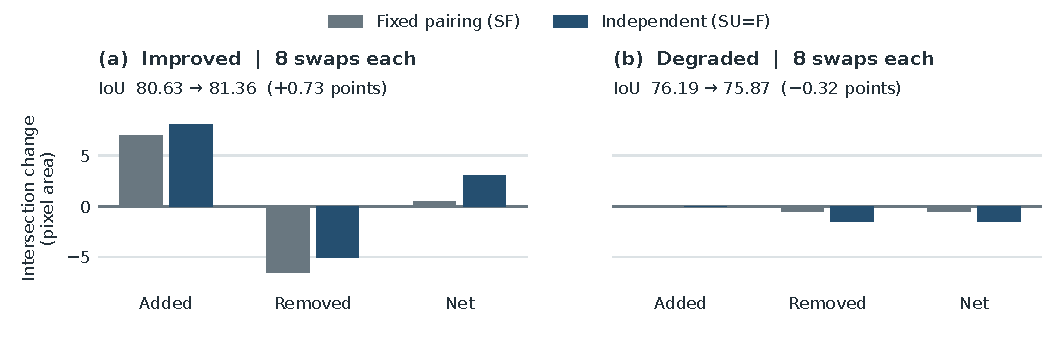
\includegraphics[width=\textwidth]{figures/dev705_overlap_cases.pdf}
\caption{Two observed RF-DETR DEV705 matches at the same edit count in seed 5217. Each arm adds eight pixels and removes eight. Bars report the intersection contributed by added native cells, the intersection lost in removed cells, and their net effect relative to the raw mask. IoU compares each complete edited mask with the same reference polygon. Cases are observed matches nearest the median within the positive and negative IoU differences, respectively, with the first image excluded when choosing the second case.}
\label{fig:dev-cases}
\end{figure*}

For seed 5217, freeing the pair assignment improves 1,012 of 1,461 fixed matches (69.3\%) and degrades 252 (17.2\%). The remaining 197 (13.5\%) differ by at most \(10^{-12}\) in continuous IoU. Fig.~\ref{fig:dev-cases} decomposes two median-sign cases using exact overlap. In (a), the independent additions recover one extra reference pixel-equivalent and the removals spare another 1.5. IoU gains 0.732 points. In (b), neither policy's additions recover any reference area. Independent selection removes one more pixel-equivalent of the hull and loses 0.316 IoU points. The second case illustrates a failure of occupancy ranking even though the independent writer maximizes estimated gain.

At each head seed's realized natural-policy counts, ranking by true pixel occupancy would improve continuous IoU by 2.111 points over SU, with a paired interval of \([1.863,2.383]\). Varying the number of additions and removals at the same total count yields an additional 1.001 points, with interval \([0.814,1.224]\). These bounds retain the 1,461 original matched objects and the same endpoint support. With learned ranks frozen, a quota-only oracle gains 1.264 points over SU. All bounds are conditional on native matches.
We trained a second RF-DETR with the same data and initialization and a different downstream seed (5203). Using its own candidates and scores and the unchanged three point heads, the matched-count policy gains 0.838 AP and 0.583 continuous IoU points over fixed pairing. The 95\% source-group IoU interval is \([0.488,0.678]\) over 1,465 fixed matches from 27 groups. Gains are positive for each head. The natural count raises AP from 55.914 to 56.726. The two detector fits share the starting weights and the evaluation images.

\subsection{Frozen Evaluation on the HRSID Official Split}
The official-split reevaluation uses the first E24 RF-DETR fit (5202), three frozen FIT109 point-head seeds, and 187,796 native mapped candidates. An independent replay verifies candidate identities, scores, realized edit counts and written masks. The natural policy gains 1.021 mask AP points over the native masks (Table~\ref{tab:official}), with seed effects of 1.078, 1.062 and 0.923 points. At the fixed-pair count, independent selection gains 1.216 AP, 1.958 AP75 and 1.379 small-object AP points. Its AP gains are 1.052, 1.297 and 1.299. Both comparisons remain positive for every seed when excluding empty annotations or exact image overlap. Their mean AP gains range from 1.018 to 1.029 and 1.207 to 1.216 points, respectively.

\begin{table}[t]
\centering
\caption{HRSID official test allocation. Refined rows are means over three point-head seeds on one frozen detector. COCO metrics are scaled by 100.}
\label{tab:official}
\footnotesize
\begin{tabular}{@{}lrrrrr@{}}
\toprule
Policy & AP & AP75 & AP90 & Small AP & AR100\\
\midrule
N & 54.433 & 62.190 & 4.417 & 52.823 & 61.694\\
SF & 54.227 & 61.862 & 4.307 & 52.570 & 61.179\\
SU=F & 55.444 & 63.821 & 4.908 & 53.949 & 62.790\\
SU & 55.454 & 63.709 & 4.925 & 53.960 & 62.774\\
LW=S & 55.130 & 63.260 & 4.827 & 53.591 & 62.265\\
\bottomrule
\end{tabular}
\end{table}

Relative to LW=S, SU gains 0.324 AP points on average, with seed effects of \(+0.184\), \(+0.963\), and \(-0.174\). This contrast changes both the predictor and area policy. Switching from SU=F to the natural count changes mean AP by \(+0.011\) and AP75 by \(-0.112\) points. The official comparison supports a recurring cost of distance-based pairing on carrier 5202 (Fig.~\ref{fig:transfer-effects}). On this split the independent replay establishes COCO AP. Source and transfer analyses supply the fixed-match continuous effects.

\begin{figure*}[!t]
\centering
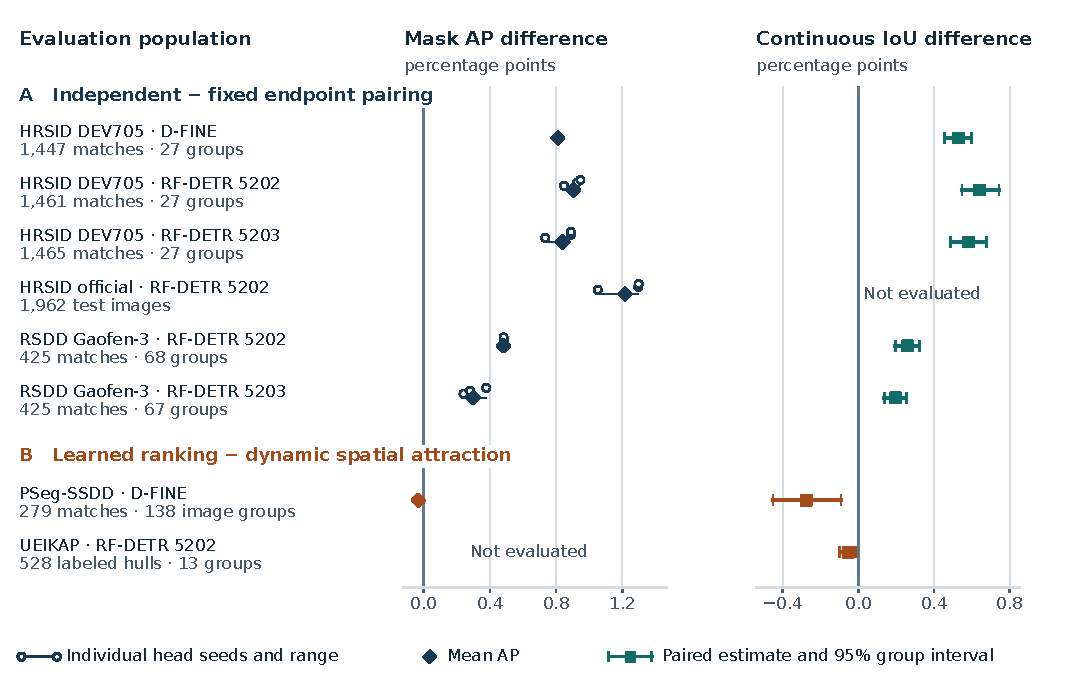
\includegraphics[width=\textwidth]{figures/transfer_effects.pdf}
\caption{Matched-budget effects across cohorts. In (A), independent selection is compared with fixed pairing using the same point head, candidate and realized count. AP symbols show observed head-seed effects and their mean. IoU intervals come from resampling the represented groups. In (B), learned ranking is compared with dynamic attraction at identical realized counts. PSeg-SSDD excludes ten overlapping images. UEIKAP assigns zero change to unmatched hulls and reports no whole-scene AP. Each detector fit establishes its own native matches.}
\label{fig:transfer-effects}
\end{figure*}

\subsection{Frozen Transfer to Instance-RSDD}
Instance-RSDD~\cite{rsdd} supplies hull outlines for RSDD-SAR imagery~\cite{rsddsar}. The author files contain 2,810 training and 740 test chips, compared with 2,840 and 715 in the paper. The 740 test chips contain 872 outlined vessels, and all 112 test parent scenes recur in the author training allocation. Our models are fitted on HRSID only. The prespecified Gaofen-3 view represents a sensor absent from HRSID fitting (583 chips, 631 outlines and 76 acquisitions). The remaining 157 test chips are TerraSAR-X.

On Gaofen-3, the first detector's two natural policies gain 0.587 and 0.517 AP over native. AP75 rises by 1.438 and 1.230, while AP90 falls by 0.094 and 0.107. With count fixed, the corresponding AP gains over pairing are 0.482 and 0.483. Mean continuous IoU gains 0.259 points (\([0.194,0.322]\), 425 eligible matches, 68 contributing acquisitions). This is a paired mean over the two heads. The second detector, sharing initialization and point-head provenance, gains 0.240, 0.280, and 0.378 AP points at equal count. Its mean AP and IoU gains are 0.299 and 0.196 (\([0.136,0.253]\)) on its own 425 eligible matches, with 67 contributing acquisitions. Across all 740 images, natural selection gains mean AP of 0.539 and 0.435 for the two fits. The gain from freeing pairs at fixed count repeats more consistently than a large improvement over the native proposal.

The separate reserve contains 74 chips from 13 additional parents in the author training allocation. With detector 5202 and head 5217, equal-count independence gains 0.436 AP and 0.318 IoU (\([0.217,0.436]\), 47 eligible matches). The nested date-separated view contains 42 chips and 32 eligible matches. It gains 0.840 AP and 0.364 IoU (\([0.250,0.478]\)). Detector 5203 has 48 and 31 eligible matches in the two views. Its three-head means gain 0.306 and 0.529 AP and 0.267 and 0.326 IoU (\([0.161,0.374]\), \([0.166,0.460]\)). Both fits meet the 20-match and eight-parent criteria in each view. Intervals resample sensor--dates with equal parent weights. The date split probes temporal proximity within the reserve. Geographic independence is unverified.

\subsection{What the Ranking Changes at the Same Budget}
After fixing the edit budget, the next question is whether learned scores select better cells than a geometric rule. On the 74-chip reserve, at the dynamic attraction count, occupancy gains 0.468 AP and 0.431 IoU over dynamic (\([0.213,0.662]\)), and 0.203 AP and 0.301 IoU over static (\([0.088,0.534]\)). Static still leads by 0.173 AP75. Both contrasts change 47 eligible masks in 11 sensor--date blocks. The date-separated AP gains are 0.978 and 0.478, while neither sensor stratum alone meets the exposure criterion.

\begin{figure*}[!t]
\centering
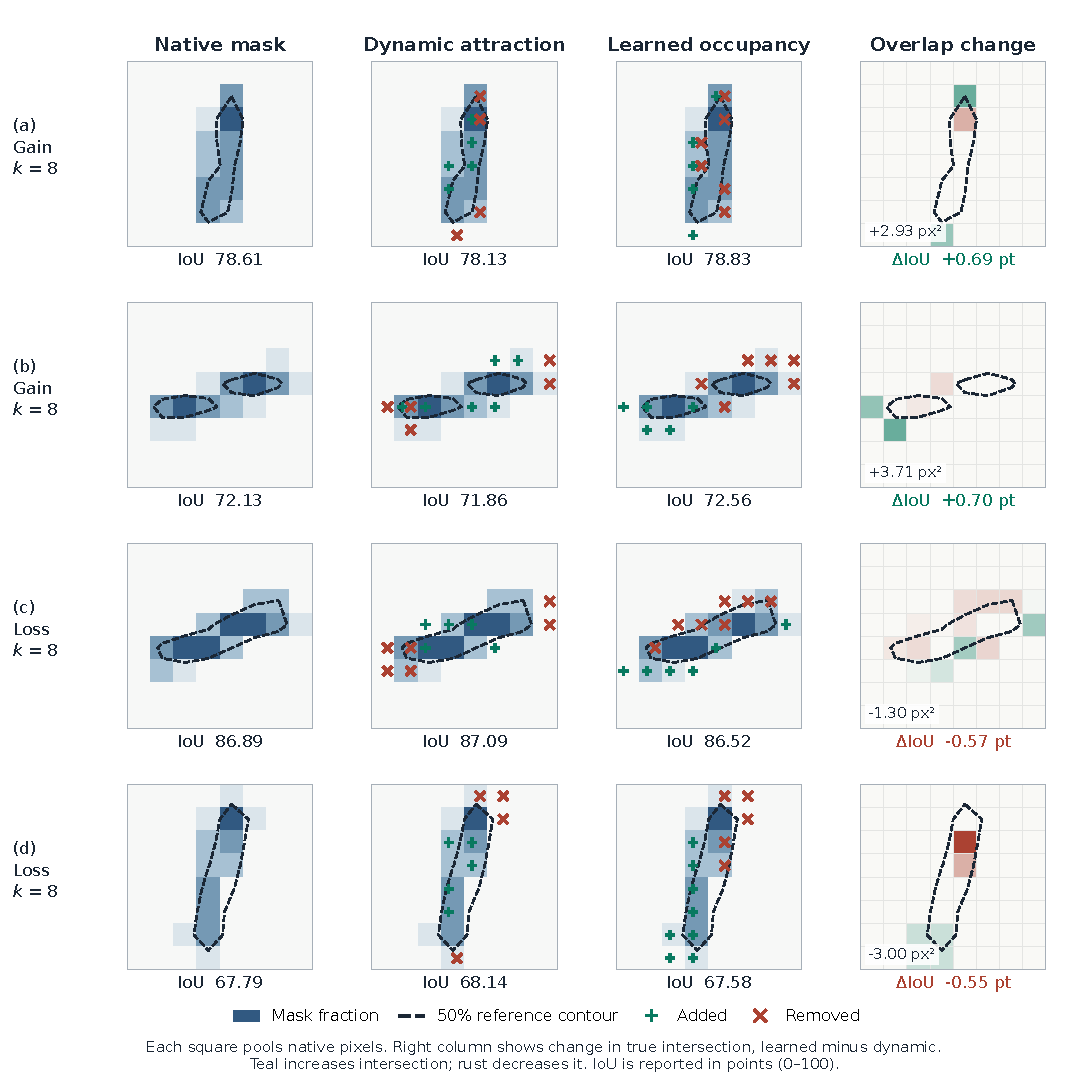
\includegraphics[width=\textwidth]{figures/gf3_matched_cases_binned.pdf}
\caption{Observed Gaofen-3 outcomes at matched dynamic-attraction counts, detector 5203 and occupancy head 5217. Two positive and two negative cases are selected by proximity to the continuous-IoU median within each sign among 425 eligible original matches, before inspection of the imagery. All illustrated edits add eight and remove eight native pixels. The public visual pools exact masks, reference coverage and signed changes to an \(8\times8\) spatial grid. The dashed binned reference can fragment a narrow footprint. Reported IoU and signed overlap are evaluated on the original grid using the author polygon.}
\label{fig:gf3-qual}
\end{figure*}

For the second detector's 425 eligible Gaofen-3 matches, seed 5217 improves 268 masks (63.1\%) over dynamic attraction, worsens 154 (36.2\%), and ties three. Fig.~\ref{fig:gf3-qual} shows where area is redistributed in four cases, all at eight swaps. In the first two, learned ranking increases net reference intersection by 2.93 and 3.71 native pixel areas over dynamic attraction. Continuous IoU rises from 78.13 to 78.83 and from 71.86 to 72.56. In the other two, equal-sized edits lose 1.30 and 3.00 pixel areas of intersection. IoU falls from 87.09 to 86.52 and from 68.14 to 67.58. The native masks provide a third reference in each row. The gains and losses measure covered polygon area on the image grid.

Strict matches are also sensitive to how the same source polygon is represented. In the second fit on Gaofen-3, learned minus dynamic AP90 changes from \(-0.149\) under standard raster overlap to \(+0.004\) under polygon--cell overlap. The paired 95\% interval for the change is \([-0.195,0.579]\). The first fit shrinks from \(+0.279\) to \(+0.053\). The 631 outlines and the prediction identities and order are held fixed. In both fits, the mean AP advantage averaged across the ten thresholds remains positive. The strict-threshold result motivates reporting the overlap convention and match coverage alongside AP90.

At matched endpoints and counts on 74 chips, five-pass Phoenix XL1~\cite{phoenix} without its 1\% gate gains 0.308 AP (58.976) and 0.135 IoU (\([-0.026,0.277]\)) over occupancy. Substituting occupancy for only the Phoenix additions changes mean AP by \(-0.012\), while substituting only deletions changes it by \(-0.225\). Both adjusted intersection intervals cross zero. Under image-only \(\pm1\)-column shifts, the mean signed centroid response is 0.117 pixels for Phoenix and 0.070 for occupancy (paired difference 0.047, \([0.028,0.064]\), 47 hulls). The latter result measures sensitivity to image alignment on fixed proposals. Its contribution to the ranking gap on correctly aligned images remains uncertain.

At fixed head and count, freeing both sides versus additions alone gained 0.224 AP and 0.175 IoU on Gaofen-3 (two-seed means, \([0.130,0.222]\)) and 0.169 AP and 0.170 IoU on the 74 chips (\([0.108,0.251]\)). Over deletions alone, gains were 0.199 AP and 0.085 IoU (\([0.049,0.120]\)) and 0.288 AP and 0.148 IoU (\([0.042,0.252]\)). AP rose at every seed. Both date-separated IoU intervals stayed positive.

\subsection{Phoenix Whole-Mask Transfer}
On the same 74 chips, we also apply the author XL1 binary writer to native masks, with its original five refinement iterations and independently evaluated area rules. The COCO rule permits only the 172 candidates with foreground exceeding 1\% of the image and skips every candidate in our 32--1023-pixel range. The LVIS rule refines all 6,079 nonempty native masks. Both rules keep the original scores and all 7,346 candidate identities. The 172 shared eligible outputs are identical. In a label-free check, thresholding the archived Phoenix probabilities at 0.50 reproduces the full-mask writer at all 259,242 recorded endpoints across 4,107 matched-budget candidates.

\begin{table}[t]
\centering
\caption{Phoenix endpoint and full-mask writers on the 74-chip Instance-RSDD reserve. Hulls count COCO rematches at IoU 0.50 among 81 references.}
\label{tab:phoenix-whole}
\footnotesize
\begin{tabular}{@{}lrrr@{}}
\toprule
Mask policy & AP & AR100 & Hulls\\
\midrule
Native RF-DETR & 58.277 & 73.457 & 81\\
Occupancy, matched count & 58.668 & 73.992 & 81\\
Phoenix, matched count & 58.976 & 73.951 & 81\\
Phoenix whole, COCO gate & 58.161 & 73.210 & 81\\
Phoenix whole, LVIS gate & 41.198 & 57.654 & 73\\
\bottomrule
\end{tabular}
\end{table}

The LVIS-policy write loses 17.779 AP points relative to matched Phoenix (Table~\ref{tab:phoenix-whole}). Continuous IoU decreases by 9.825 points (95\% interval \([-14.014,-6.440]\), 47 original eligible matches in 11 sensor--date blocks). False positive area increases by 33.726 points of reference area (\([19.461,50.351]\)), and missed area changes by \(-2.905\) points (\([-5.907,0.286]\)). Of the 81 original hull associations, 65 survive at IoU 0.50. Rematching reaches 73 hulls. In the date-separated view, AP and IoU fall by 19.137 and 11.327 points, respectively. Both sensor views have the same sign, with fewer than eight contributing date blocks per view. The effects are specific to this previously evaluated detector stream. Whole writing changes support, area and eligibility jointly.

To test area conservation under a common edit limit, we keep the same Phoenix probabilities, endpoints and \(2k\) flips for every candidate. We rank addition gains by \(p-0.50\) and removal gains by \(0.50-p\), where \(p\) is the frozen Phoenix occupancy. Sorted prefixes determine the maximum estimated pixel-correctness gain under each quota. With no constraint on \(d\), the 59,800 flips add a net 23,828 foreground cells across all predictions. Relative to that policy, strict balance gains 0.190 AP and 0.083 continuous IoU (\([-0.191,0.401]\)). The written masks differ for 45 fixed hulls in 11 sensor--date blocks. A two-cell tolerance on \(|d|\) gives 58.856 AP, compared with 58.976 for strict balance and 58.787 for free allocation. All three retain the 81 original matches. On HRSID DEV705, free allocation with a source-trained occupancy head gains 0.212 AP and 0.009 continuous IoU over balance at 631,020 fixed flips in a single fit. The estimated effect is small on the Instance-RSDD reserve and changes direction in the HRSID comparison, which also uses a different ranking field. The much larger loss under whole writing calls for separate tests of support and flip count.

\subsection{Writable Support and Edit Count}
We cross the writable support with the flip rule using the same fifth-iteration Phoenix posterior for each of the 4,107 positive-budget candidates. All other candidates retain the native mask. Narrow support uses the original sampled endpoints. Whole support covers the original image grid. The threshold writer applies the author's binary decision at every available location. Exact-count writing uses the same \(2k\) flips as the original narrow run and maximizes summed pixel-correctness gain with free signed counts. The narrow exact-count masks and the whole threshold masks reproduce their respective archived masks on all 4,107 candidates. All 259,242 recorded probabilities also match.

\begin{figure*}[!t]
\centering
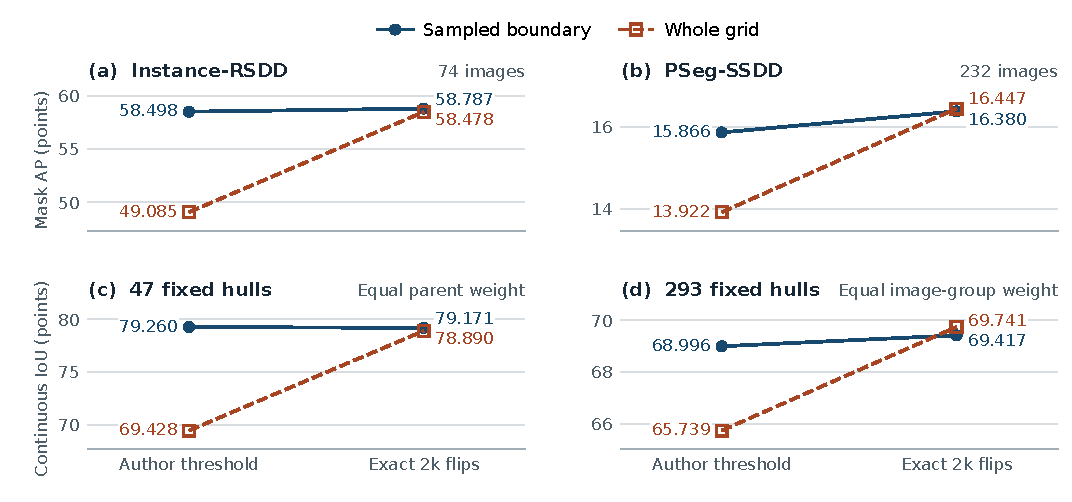
\includegraphics[width=\textwidth]{figures/phoenix_budget_by_dataset.pdf}
\caption{Writable support and edit count on two frozen detector streams. Within each dataset, all four policies use the same editable candidates and Phoenix probabilities. Mask AP uses the full native candidate stream. Continuous IoU weights parent scenes equally over 47 original eligible matches on Instance-RSDD and decoded-image groups equally over 293 matches on PSeg-SSDD. Each panel uses its own vertical scale.}
\label{fig:phoenix-support-budget}
\end{figure*}

On whole support, imposing the old count reduces flips from 2,042,908 to 59,800 and raises AP from 49.085 to 58.478 (Fig.~\ref{fig:phoenix-support-budget}). Continuous IoU increases by 9.462 points (paired 95\% interval \([6.329,13.283]\)). False positive area drops by 33.131 points of reference area (\([-49.245,-19.298]\)), and missed area changes by \(+2.957\) points (\([-0.058,5.863]\)). The number of hulls rematched at IoU 0.50 recovers from 77 to 81. The exact-count rule uses 44,158 cells outside the sampled support. Relative to native, its AP improves by 0.201 points while AR100 is 0.494 points lower.

On narrow support the count constraint changes AP by \(+0.289\) and IoU by \(-0.089\) points. The count effect is 9.105 AP points larger on whole support. The continuous-IoU interaction is 9.551 points (\([6.398,13.365]\)). The equal-count comparison of narrow and whole writing gives \(+0.309\) AP and \(+0.281\) IoU for the narrow writer, with interval \([-0.025,0.666]\). On the 42 date-separated chips, the whole-support count effect remains positive at 12.920 AP and 10.672 IoU points.

On PSeg-SSDD, we switch to frozen D-FINE and keep the original dynamic-attraction counts on the 11,054 editable candidates. The whole-grid threshold writer performs 3,391,327 flips. The exact-count writer performs 147,540, raising AP from 13.922 to 16.447 and fixed continuous IoU by 4.001 points (\([2.644,5.382]\)). Foreground outside the reference falls by 7.382 points of reference area (\([-11.989,-3.621]\)). At IoU 0.50, rematching covers 404 hulls instead of 407, and the number retaining their original candidate rises from 377 to 394. On 222 images after excluding historical exact overlaps, AP and continuous IoU rise by 2.694 and 4.095 points under the same count comparison. All comparisons retain the official allocation's full candidate stream for the applicable images.

The narrow exact-count writer on PSeg-SSDD improves on narrow thresholding by 0.514 AP and 0.422 IoU points (\([0.253,0.595]\)). At the fixed count it scores 0.067 AP lower than the whole writer and loses 0.323 IoU points (\([-0.560,-0.111]\)). The count effect on whole support exceeds the effect on narrow support by 2.011 AP and 3.580 IoU points (IoU interval \([2.316,4.887]\)). Applying the bound therefore reduces threshold-write errors in both datasets, with different residual errors. On PSeg-SSDD, whole-support exact-count Phoenix remains 1.528 AP below native D-FINE and 1.970 AP below matched static attraction.

At the same 147,540 flips on the sampled endpoints, assigning half to each side raises Phoenix AP from 16.380 to 18.222 on PSeg-SSDD. The paired continuous IoU gain is 1.151 points (\([0.701,1.594]\)). The writers differ on 283 of 293 fixed matches and in 137 of 143 decoded-image groups. Missed area falls by 1.428 points of reference area and false-positive area rises by 0.340 points. The balanced writer trails matched static attraction by 0.195 AP and 0.076 IoU points (\([-0.246,0.105]\)). Compared with the matched learned head, it gives 0.109 lower AP and 0.186 higher IoU (\([0.036,0.339]\)). After excluding ten historical exact overlaps, the balanced writer gains 2.093 AP and 1.232 IoU points over free allocation (\([0.762,1.682]\)). The matched differences relative to static and learned rankings retain their directions.

\begin{figure*}[!t]
\centering
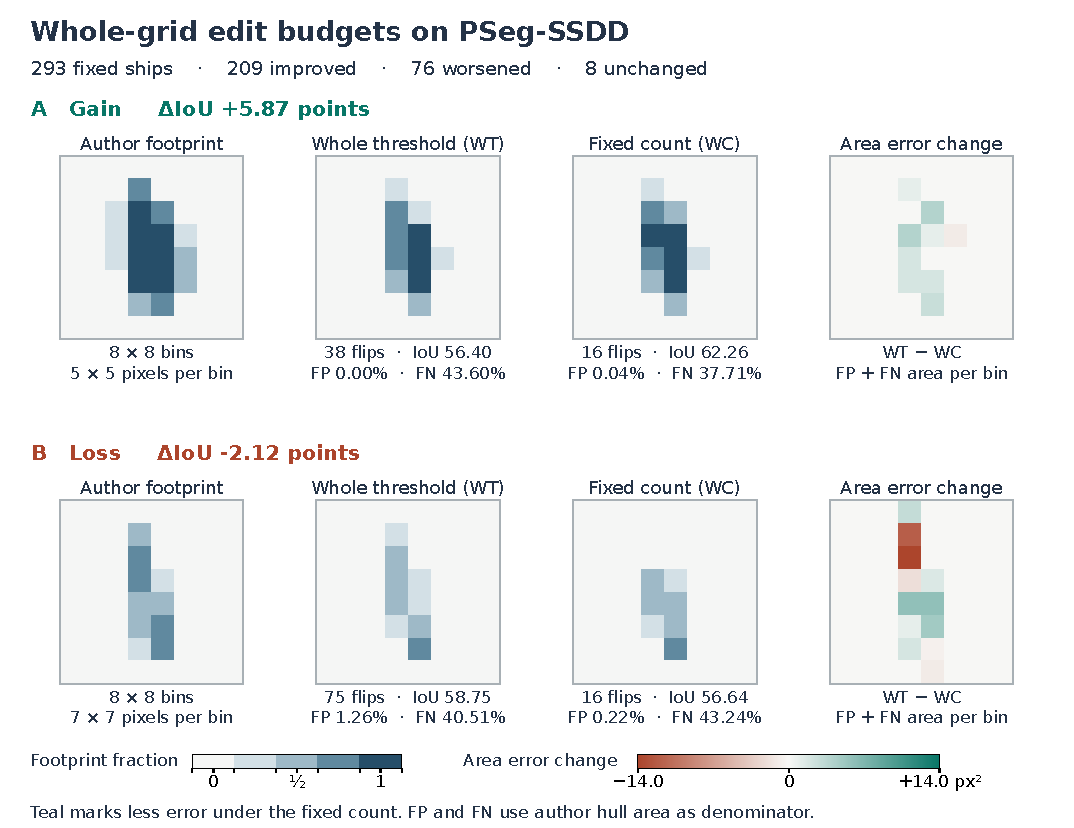
\includegraphics[width=\textwidth]{figures/pseg_budget_cases_binned.pdf}
\caption{Observed gain and loss from limiting the number of whole-grid writes on PSeg-SSDD. Two distinct images were selected near the respective sign-specific medians of continuous-IoU change before inspection. Columns show pooled reference occupancy, the threshold and fixed-count footprints, and the change in area error. The error map is threshold minus fixed count, where teal indicates lower error at the fixed count. False-positive and false-negative percentages and IoU use the original polygon and cell grid.}
\label{fig:pseg-budget-cases}
\end{figure*}

The whole-support count improves 209 of the 293 original eligible PSeg matches, worsens 76, and ties eight. In Fig.~\ref{fig:pseg-budget-cases}(A), the threshold output shrinks inward along the sides of the hull. Reducing 38 flips to 16 retains an additional \(17.87\) native pixel areas inside the reference, raising IoU from 56.40 to 62.26. The native mask has IoU 66.88. In (B), thresholding restores part of the narrow upper end and increases IoU from 56.04 to 58.75. Sixteen fixed-count changes reduce the false-positive fraction from 1.26\% to 0.22\% and lose \(7.96\) pixel areas of reference intersection, giving IoU 56.64.

\subsection{Source-Fitted PointRend on Instance-RSDD}
Binary PointRend used HRSID FIT109 RF-DETR features, 200 updates at 196 targets/update, 3,136 evaluations/RoI and zero padding. Both heads ranked capped or complete two-layer box support at seed 5217 occupancy counts with row-major ties. Their features and supervision differed.

\begin{table}[t]
\centering
\caption{Gaofen-3, frozen RF-DETR. Both rankings exchange 268,347 pairs across 34,808 candidates. IoU weights acquisitions equally over 425 fixed matches. All scores are points.}
\label{tab:rsdd-pointrend}
\setlength{\tabcolsep}{4pt}
\begin{tabular}{lrrrr}
\toprule
Policy & AP & AP75 & AP90 & IoU\\
\midrule
Native RF-DETR & 61.033 & 71.822 & 3.256 & 79.652\\
Coarse RoI paste & 53.880 & 56.474 & 1.486 & 75.108\\
PointRend RoI paste & 61.831 & 74.396 & 3.227 & 79.939\\
\midrule
PointRend ranks, capped & 61.309 & 72.646 & 3.017 & 79.647\\
Occupancy ranks, capped & 61.620 & 73.259 & 3.162 & 79.897\\
PointRend ranks, complete & 61.241 & 72.525 & 3.015 & 79.648\\
Occupancy ranks, complete & 61.631 & 73.280 & 3.041 & 79.871\\
\bottomrule
\end{tabular}
\end{table}

Against PointRend, occupancy gains 0.312 AP and 0.250 IoU on capped support (\([0.163,0.338]\)), and 0.390 AP and 0.223 IoU on complete support (\([0.123,0.330]\), Table~\ref{tab:rsdd-pointrend}). Removing the cap changes these gaps by \(+0.078\) AP and \(-0.027\) IoU (\([-0.086,0.028]\)).

Full paste gains 0.200 AP over complete-support occupancy but lowers AR100 (72.361 vs.\ 74.105). Outside capped support lie 90.6\% of its differences from capped PointRend ranks. Capped paste scores 61.782 AP and 73.566 AR100 at unequal counts. On complete support, 25.2\% of PointRend and 3.4\% of occupancy deletions lie outside the RoI. The matched results compare two rankings of available endpoints. The paste also changes which cells are available and how much area is written, making its AP and recall relevant to a separate system-level decision.

Inside the clipped RoI (268,302 exchanges), occupancy gains 0.379 AP and 0.224 IoU with zero padding (\([0.125,0.329]\)), and 0.345 AP and 0.223 IoU with border replication (\([0.124,0.327]\)). Padding accounts for 0.034 AP and 0.001 IoU (\([-0.006,0.008]\)).

At 31,391 exchanges, occupancy beat capped PointRend by 0.477 AP and 0.395 IoU on the 74 chips (\([0.204,0.620]\)). Date-separated gains were 1.061 AP and 0.490 IoU (\([0.225,0.751]\)).

Preserving PointRend outside capped support and its per-mask signed counts, occupancy raised AP at all three seeds. Mean AP rose from 57.534 to 58.196 on the 74 chips and from 61.831 to 61.975 on Gaofen-3. IoU gained 0.251 (\([0.051,0.449]\)) and 0.195 (\([0.109,0.281]\)). Locations differed on 44/47 matches in 12 parents and 424/425 in 68 acquisitions. We averaged seeds per match for 4,096 paired sensor--date draws (equal parents) or acquisition draws (equal acquisitions). Date-separated gains were 0.781 AP and 0.284 IoU (\([-0.007,0.528]\)). Standalone capped occupancy scored 58.827 AP on the 74 chips.

\subsection{Source-Domain Controls}
Query features gain 0.352 AP and 0.073 IoU at fixed FIT109 counts. The IoU interval crosses zero. Zero padding and within-candidate permutation each give higher AP.

Five group-held-out FIT109 PointRend heads (200 updates each) gain 2.440 full-paste AP over coarse paste, 3.851 below native. At equal counts, balanced independent editing gains 1.047 AP and 0.262 IoU over fixed pairs (\([0.131,0.406]\)), and 0.938 AP and 0.084 IoU over unconstrained-area editing (\([-0.039,0.202]\)). The detector trained on FIT.

On HRSID FIT36, five registered shift views share the original queries, native support, 166 fixed matches and 1,209 swaps. The second-worst signed rank loses 0.333 continuous IoU points to the mean-logit rank (\([-0.489,-0.149]\)).

\subsection{Frozen Transfer to PSeg-SSDD}
Five frozen HRSID policies share all 18,700 native candidates, including empty masks (Table~\ref{tab:ssdd}).

\begin{table}[t]
\centering
\caption{Frozen HRSID-to-PSeg-SSDD mask AP on DEV187. Float and integer use 187 images. Dedup.\ scores float polygons on 182 unique decoded images.}
\label{tab:ssdd}
\footnotesize
\begin{tabular}{@{}lrrr@{}}
\toprule
Mask policy & Float & Integer & Dedup. \\
\midrule
Raw D-FINE E24 & 17.897 & 16.804 & 18.261 \\
Same head, fixed pairing & 17.956 & 16.877 & 18.329 \\
Independent, fixed-policy count & 18.028 & 17.173 & 18.393 \\
Independent, natural count & \textbf{18.234} & \textbf{17.557} & \textbf{18.620} \\
Native ranks, natural-policy count & 17.942 & 16.757 & 18.308 \\
\bottomrule
\end{tabular}
\end{table}

On DEV187, natural selection gains 0.336 AP over native and 0.278 over fixed pairing, below the 0.50 and 0.30 margins. At equal counts, independent selection gains 0.071 AP and 0.112 IoU (\([0.048,0.178]\), 209 fixed matches, 111 image groups). No match exceeds 0.90. Deduplication preserves the directions. Acquisition independence remains unverified.

On the historical official split, AP rises from 17.974 to 18.319 and AP75 from 13.015 to 14.705. At equal counts, AP exceeds fixed pairing by 0.081. Ten test images share decoded content with the historical PSeg training allocation. Excluding them yields 0.389 AP over native and 0.100 over fixed pairing. The detector and head in this transfer comparison were fitted on HRSID.

Across 293 editable matches, independent selection gains 0.106 IoU over fixed pairs (image-paired 95\% interval \([0.055,0.157]\)). Natural selection gains 0.228 over native (\([0.104,0.364]\)). All stay below 0.90. Oracle ranks at the learned count add 1.097 IoU points. Allowing unequal counts at the same total flips adds 2.020 more.

At the dynamic attraction count~\cite{atkinson} (73,770 exchanges, 11,054 predictions), learned ranking scores 18.331 versus 18.357 AP, gains 0.279 AP75 and loses 0.270 IoU (\([-0.440,-0.098]\)). Deduplication preserves these directions. Releasing the distance assignment helps the occupancy writer at its paired count. At the dynamic count, the same occupancy scores produce lower continuous overlap than attraction.

\subsection{Source and Target Heads on a PSeg-Trained RF-DETR}
At the dynamic edit count on historical DEV187, the transferred HRSID head scores 69.958 AP, and dynamic attraction scores 69.113 with the same PSeg-trained RF-DETR E24. The 0.193 IoU gain misses the criterion (119-group paired 95\% interval \([-0.036,0.430]\)). Native masks score 70.694 AP, leading by 0.735 AP and 0.404 IoU (\([0.245,0.564]\)). Equal-count independent selection gains 0.279 AP and 0.097 IoU over fixed pairing (\([-0.035,0.232]\)).

On 281 matches, polygon-optimal ranks at the attraction count exceed native by 2.246 IoU and learned ranks by 2.651. Fewer flips on frozen support add 0.032 beyond this optimum, and varying area at fixed total flips adds 1.018. These reference-dependent ceilings identify recoverable overlap inside the evaluated support, with scope to improve both the rankings and the area constraint.

Refitting on 109 PSeg training images (zero decoded DEV187 overlap, 200 updates) yields 69.809 AP at the attraction count, 0.695 above dynamic, 0.150 below transfer and 0.885 below native. IoU falls 0.470 from native (\([-0.621,-0.325]\)). Deduplicated AP agrees in direction. The refit misses the replication criterion.

\subsection{Frozen Transfer to Sentinel-1 Acquisitions}
UEIKAP~\cite{ueikap} supplied 139 hulls on 108 chips from 18 acquisitions. The evaluation required 20 positive-budget IoU-0.50 matches across eight acquisitions. D-FINE matched two at zero budget (eight ideal swaps could cover four). HRSID RF-DETR had 17 positive-budget matches in four groups. Independent selection gained 0.515 IoU points over equal-count fixed pairing conditional on those four represented groups. Assigning zero change to unmatched hulls gives 0.03014 points across all 18 groups (paired 95\% interval \([0.00028,0.08025]\)). All 17 remained below 0.75.

RF-DETR boxes reached IoU 0.50 for 100 hulls. In 90, the mask associated with the highest-overlap box had total foreground area below half the reference area. The median area ratio was 0.301. Geometric ceilings reached IoU 0.50 for 18 hulls with eight ideal swaps and 129 with within-box reconstruction. These are per-hull ceilings that allow candidate reuse. Score-ordered box matching selected 99 sub-0.50 masks (90 positive budgets, 15 acquisitions). Equal-count selection gained 0.0043 IoU across 18 acquisitions (\([-0.0008,0.0101]\)). None reached 0.50. Box and mask matching selected different candidates for 16 of 17 shared hulls. The area deficit and association changes limit the hulls accessible to a small, area-preserving edit.

Across 342 chips from 13 additional Danish acquisitions, RF-DETR matched 121 of 528 released hulls. Positive budgets on 120 matches in ten groups met the criterion. Equal-count independent selection gained 0.02954 IoU over fixed pairing (group-equal 95\% interval \([0.00790,0.05198]\), unmatched hulls counted as zero), and 0.12306 among matches (\([0.02106,0.21932]\)). Learned ranking lost 0.05322 IoU to dynamic attraction at its count (\([-0.09777,-0.01562]\)). Natural selection gained 0.00623 over native (\([-0.02481,0.03017]\)). One fixed match reached continuous IoU 0.75 under every local policy.

On these previously evaluated chips, the frozen FIT109 PointRend head refined native masks of area \([32,1024)\) pixels. At raster IoU 0.50, native masks, \(7{\times}7\) coarse pastes and \(224{\times}224\) PointRend pastes covered 121, 111 and 30 case-focused hulls, respectively. PointRend recovered no new hulls against either comparator and omitted more hull area at fixed box associations, losing 4.1375 continuous IoU points to native and 3.4553 to coarse across all 528 hulls.

\subsection{Addition and Removal Locations Across Cohorts}
At the dynamic edit count, replacing static attraction with learned additions or removals alone changed true intersection (\% of hull area) by \(+0.308\) and \(+0.446\) points on HRSID DEV705, and \(-0.082\) and \(-0.076\) on PSeg-SSDD TEST232 (same D-FINE). RF-DETR gave \(-0.02157\) and \(-0.01466\) on UEIKAP342. Adjusted 97.5\% intervals excluded zero for PSeg removals and UEIKAP additions. Both external 95\% intervals for additions minus removals crossed zero, leaving the dominant side unresolved.

\begin{samepage}
A \href{https://github.com/bingzhi495-creator/SAR-SEAL-research/blob/3f8f738/research_round_20260925_global/ATTRACTION_LOCAL_CORRECTION_ACTUAL_20261123.md}{ridge model} fit on 4,063 FIT109 pairs chose between disputed static and learned locations. On historical D-FINE DEV705 it gained 0.01795 IoU over scores alone at equal accepted counts per mask and sign (paired 95\% interval \([0.00796,0.02803]\)). Against learned ranks alone it gained 0.051 AP. On 222 deduplicated PSeg images, matched-count IoU gained 0.01567 (\([-0.00334,0.03754]\)), and static attraction led by 0.11484 AP and 0.16918 IoU.\par
\end{samepage}

\section{Discussion and Reproducibility}
\subsection{Transfer and Proposal Coverage}
On Gaofen-3, releasing the pairing constraint improves AP and fixed-match IoU across the two RF-DETR fits. The fits share evaluation scenes and initialization, so the comparison assesses repeatability across downstream fitting on the same cohorts. On PSeg-SSDD, replacing dynamic attraction with learned ranks at its realized count lowers continuous IoU. Even with the same attainable set of edited masks, source scores can order their cells differently from the target polygons.

On both historical datasets, capping whole-image Phoenix edits reduces exterior false-positive area. On PSeg-SSDD, all four support-by-count policies trail the native detector. The additional narrow, balanced policy slightly exceeds the native AP and nearly closes the gap to static attraction. This recovery shows that a total edit count can leave a substantial difference in the allocation of corrections to foreground and background. The same constraint produces a smaller, uncertain effect on Instance-RSDD. These experiments change both the detector and the image population between datasets. On the UEIKAP reserve, only 17 of 139 released hulls have positive-budget native matches. The within-box reconstruction ceiling suggests that usable proposals matter before local correction.

The HRSID official set was used during earlier development. Gaofen-3 intervals resample released acquisitions. For the 74-chip Instance-RSDD reserve we weight parent scenes equally and resample sensor--date blocks. PSeg intervals instead resample decoded-image groups because acquisition identities are unresolved. These protocols delimit the evidence and leave performance on geographically independent acquisitions open.

\subsection{Topology and Physical Measurements}
Area preservation leaves topology unconstrained. On DEV705 an edit can improve overlap with the intended hull and simultaneously increase overlap with a neighbor. Natural selection increased the hole count in 1,544 of 10,466 edited PSeg masks. Writing the same counts with native ranks did so in 519. All 107 nonempty D-FINE masks in the Schwegmann set~\cite{schwegmann} were below the 32-pixel size floor. These observations constrain applications that require connected hulls or very small instances.

Of 142 NovaSAR AIS chips~\cite{nastar}, 34 yielded common spans across policies and 17 had positive edit budgets. Equal-count independence increased absolute length error by 0.204\,m over fixed pairing (\([-0.110,0.581]\)\,m). In the Gulf set~\cite{gulf}, 242 of 244 chips from 64 Sentinel-1A orbit--dates passed input checks. The AIS association and common-span criteria retained 25 ships in 19 groups, of which 23 had positive edit budgets. Native span bias was 105.42\,m at nominal spacing and 107.05\,m after geolocation. Equal-count independent selection reduced nominal MAE by 0.168\,m (\([-1.523,1.692]\)\,m). In the 23 cases with headings, comparison on that same subset shows that using AIS heading reduced geolocated MAE by 7.60\,m (\([1.88,14.89]\)\,m), leaving 71.27\,m mean excess. The magnitude of residual error limits the use of these mask edits for physical sizing.

\subsection{Computation and Repeatability}
D-FINE ran 24 epochs (17,640 updates). Its CUDA detector and postprocessor took 11.74\,s over the 232 PSeg images in one run. With those inputs already loaded, exact-equivalent interpolation reduced single-thread refinement from 158.8 to 104.3\,ms/image. On the 74 Instance-RSDD chips, occupancy writing, equal-count PointRend and whole-RoI PointRend took 227.1, 1,221.5 and 1,049.2\,ms/image, respectively, over two single-thread passes on an Intel i7-13700KF. These timings cover refinement after feature capture and detection. The PointRend hybrid also renders the whole RoI. The PSeg Phoenix run took 1,404.48\,s using four two-thread CPU workers for five refinement iterations on each of 11,054 prompts.

The \href{https://github.com/bingzhi495-creator/SAR-SEAL-research}{repository} provides code, configuration, score summaries and data access instructions. Independent frozen replays reproduced 3,434 numerical entries across the HRSID official and Instance-RSDD 740-chip tables. The clean 74-chip replay used detector 5202 with head 5217 and reproduced 1,470 numerical entries. A frozen replay requires access to the imagery and annotations and the corresponding checkpoints from the project owner.

\section{Conclusion}
With scores and signed counts fixed, independent selection improves AP over distance pairing on the evaluated HRSID and Instance-RSDD splits. Fixed-match IoU improves on DEV705 and the evaluated Instance-RSDD cohorts. Capping whole-image Phoenix edits reduces exterior foreground on Instance-RSDD and PSeg-SSDD. The separate addition and removal quotas also matter on PSeg-SSDD, where a balanced narrow writer recovers most of the AP gap to matched static attraction. These effects concern existing detections. On the UEIKAP reserve, few hulls enter the editable matched population.

\noindent\emph{Acknowledgment.} OpenAI Codex assisted with drafting and revision. Fig.~\ref{fig:native-boundary} was redrawn as an editable vector graphic from a generated concept. The other figures use observed results, including spatially pooled measurements in Figs.~\ref{fig:gf3-qual} and~\ref{fig:pseg-budget-cases}.


\begin{thebibliography}{26}
\bibitem{gao2024} F. Gao, X. Han, J. Wang, J. Sun, A. Hussain, and H. Zhou, ``SAR ship instance segmentation with dynamic key points information enhancement,'' \emph{IEEE J. Sel. Topics Appl. Earth Observ. Remote Sens.}, vol. 17, pp. 11365--11385, 2024. \href{https://doi.org/10.1109/JSTARS.2024.3383779}{10.1109/JSTARS.2024.3383779}.
\bibitem{aranet} S. Chang, P. Lang, H. Chang, C. Zhao, J. Yang, J. Dong, and X. Fu, ``ARANet: A unified representation alignment framework for SAR ship instance segmentation,'' \emph{IEEE J. Sel. Topics Appl. Earth Observ. Remote Sens.}, vol. 19, pp. 28679--28694, 2026. \href{https://doi.org/10.1109/JSTARS.2026.3720719}{10.1109/JSTARS.2026.3720719}.
\bibitem{drsnet} Q. Zhang and Z. Han, ``DRSNet: Rotated-ROI ship segmentation for SAR images based on dual-scale cross attention,'' \emph{IEEE Geosci. Remote Sens. Lett.}, vol. 21, pp. 1--5, 2024. \href{https://doi.org/10.1109/LGRS.2024.3420251}{10.1109/LGRS.2024.3420251}.
\bibitem{hrsid} S. Wei, X. Zeng, Q. Qu, M. Wang, H. Su, and J. Shi, ``HRSID: A high-resolution SAR images dataset for ship detection and instance segmentation,'' \emph{IEEE Access}, vol. 8, pp. 120234--120254, \href{https://doi.org/10.1109/ACCESS.2020.3005861}{2020}.
\bibitem{pointrend} A. Kirillov, Y. Wu, K. He, and R. Girshick, ``PointRend: Image segmentation as rendering,'' in \emph{Proc. IEEE/CVF Conf. Comput. Vis. Pattern Recognit. (CVPR)}, 2020, pp. 9799--9808.
\bibitem{bpr} C. Tang, H. Chen, X. Li, J. Li, Z. Zhang, and X. Hu, ``Look closer to segment better: Boundary patch refinement for instance segmentation,'' in \emph{Proc. IEEE/CVF Conf. Comput. Vis. Pattern Recognit. (CVPR)}, 2021, pp. 13926--13935.
\bibitem{refinemask} G. Zhang, X. Lu, J. Tan, J. Li, Z. Zhang, Q. Li, and X. Hu, ``RefineMask: Towards high-quality instance segmentation with fine-grained features,'' in \emph{Proc. IEEE/CVF Conf. Comput. Vis. Pattern Recognit. (CVPR)}, 2021, pp. 6861--6869.
\bibitem{sharpcontour} C. Zhu, X. Zhang, Y. Li, L. Qiu, K. Han, and X. Han, ``SharpContour: A contour-based boundary refinement approach for efficient and accurate instance segmentation,'' in \emph{Proc. IEEE/CVF Conf. Comput. Vis. Pattern Recognit. (CVPR)}, 2022, pp. 4392--4401.
\bibitem{segfix} Y. Yuan, J. Xie, X. Chen, and J. Wang, ``SegFix: Model-agnostic boundary refinement for segmentation,'' in \emph{Proc. Eur. Conf. Comput. Vis. (ECCV)}, 2020, pp. 489--506.
\bibitem{phoenix} B. Kim and S. J. Hwang, ``Learning from adversity: Semantic-aware mask refinement through adversarial perturbation,'' in \emph{Proc. Eur. Conf. Comput. Vis. (ECCV)}, 2026, pp. 75--92. \href{https://doi.org/10.1007/978-3-032-37520-9_5}{10.1007/978-3-032-37520-9\_5}.
\bibitem{atkinson} P. M. Atkinson, ``Sub-pixel target mapping from soft-classified, remotely sensed imagery,'' \emph{Photogramm. Eng. Remote Sens.}, vol. 71, no. 7, pp. 839--846, 2005. \href{https://doi.org/10.14358/PERS.71.7.839}{10.14358/PERS.71.7.839}.
\bibitem{xu} Y. Xu and B. Huang, ``A spatio-temporal pixel-swapping algorithm for subpixel land cover mapping,'' \emph{IEEE Geosci. Remote Sens. Lett.}, vol. 11, no. 2, pp. 474--478, 2014. \href{https://doi.org/10.1109/LGRS.2013.2268153}{10.1109/LGRS.2013.2268153}.
\bibitem{rankseg} B. Dai and C. Li, ``RankSEG: A consistent ranking-based framework for segmentation,'' \emph{J. Mach. Learn. Res.}, vol. 24, no. 224, pp. 1--50, 2023. \href{https://www.jmlr.org/papers/v24/22-0712.html}{Journal article}.
\bibitem{gldet} H. Chang, X. Fu, P. Lang, K. Guo, J. Dong, and S. Chang, ``GLDet: Real-time SAR ship detector based on global semantic information enhancement and local gradient information mining,'' \emph{IEEE Trans. Geosci. Remote Sens.}, vol. 63, Art. no. 5209020, 2025. \href{https://doi.org/10.1109/TGRS.2025.3559551}{10.1109/TGRS.2025.3559551}.
\bibitem{dacf} S. Yang, X. Zhang, W. An, Z. Li, and N. Chen, ``DACF-Net: A dynamic attention and context fusion network with geometry-aware multi-scale refinement for SAR ship instance segmentation,'' \emph{Int. J. Digit. Earth}, vol. 19, no. 2, Art. no. 2696657, 2026. \href{https://doi.org/10.1080/17538947.2026.2696657}{10.1080/17538947.2026.2696657}.
\bibitem{gcie} W. Luo, J. Lan, Y. Zeng, and W. Xiong, ``GCIE-Net: A global and channel information-enhanced network for ship instance segmentation in SAR images,'' \emph{Remote Sens.}, vol. 18, no. 15, Art. no. 2512, 2026. \href{https://doi.org/10.3390/rs18152512}{10.3390/rs18152512}.
\bibitem{dsr} S.-W. He, W. Xiong, and L.-B. Yao, ``SAR ship instance segmentation method in complex scenes jointly driven by differential physical fields and structured graph reasoning,'' \emph{Acta Electronica Sinica}, pp. 1--11, 2026. \href{https://doi.org/10.12263/DZXB.20260699}{10.12263/DZXB.20260699}.
\bibitem{dfine} A. Saakyan and D. Solntsev, ``D-FINE-seg: Object detection and instance segmentation framework with multi-backend deployment,'' \href{https://arxiv.org/abs/2602.23043}{arXiv:2602.23043}, 2026.
\bibitem{rfdetr} I. Robinson, P. Robicheaux, M. Popov, D. Ramanan, and N. Peri, ``RF-DETR: Neural architecture search for real-time detection transformers,'' in \emph{Proc. Int. Conf. Learn. Represent. (ICLR)}, 2026.
\bibitem{ssdd} T. Zhang \emph{et al.}, ``SAR Ship Detection Dataset (SSDD): Official release and comprehensive data analysis,'' \emph{Remote Sens.}, vol. 13, no. 18, Art. no. 3690, 2021. \href{https://doi.org/10.3390/rs13183690}{10.3390/rs13183690}.
\bibitem{rsdd} X. Yang, Q. Zhang, Q. Dong, Z. Han, X. Luo, and D. Wei, ``Ship instance segmentation based on rotated bounding boxes for SAR images,'' \emph{Remote Sens.}, vol. 15, no. 5, Art. no. 1324, \href{https://doi.org/10.3390/rs15051324}{2023}.
\bibitem{rsddsar} C. Xu \emph{et al.}, ``RSDD-SAR: Rotated ship detection dataset in SAR images,'' \emph{J. Radars}, vol. 11, no. 4, pp. 581--599, 2022. \href{https://doi.org/10.12000/JR22007}{10.12000/JR22007}.
\bibitem{ueikap} A. Mazzeo \emph{et al.}, ``UEIKAP dataset,'' Zenodo, ver. 1.0, \href{https://doi.org/10.5281/zenodo.18391027}{2026}.
\bibitem{schwegmann} C. P. Schwegmann, W. Kleynhans, B. P. Salmon, L. W. Mdakane, and R. G. V. Meyer, ``Very deep learning for ship discrimination in Synthetic Aperture Radar imagery,'' in \emph{Proc. IEEE Int. Geosci. Remote Sens. Symp. (IGARSS)}, 2016, pp. 104--107. \href{https://doi.org/10.1109/IGARSS.2016.7729017}{10.1109/IGARSS.2016.7729017}.
\bibitem{nastar} B. Hosseiny, K. Kamirul, O. Pappas, and A. Achim, ``NASTaR: A NovaSAR-based automated ship target recognition dataset,'' \emph{IEEE Geosci. Remote Sens. Lett.}, vol. 23, Art. no. 1502605, 2026. \href{https://doi.org/10.1109/LGRS.2026.3679941}{10.1109/LGRS.2026.3679941}.
\bibitem{gulf} M. Shaya, ``SAR Ship Gulf: Sentinel-1 GRD ship chips with AIS labels,'' Zenodo, ver. 1, 2026. \href{https://doi.org/10.5281/zenodo.21000650}{10.5281/zenodo.21000650}.
\end{thebibliography}
\end{document}

